\subsection{Log-domain Pulse Integrator}\label{sec:log_domain_pulse_integrator}

\begin{figure}
    \centering
    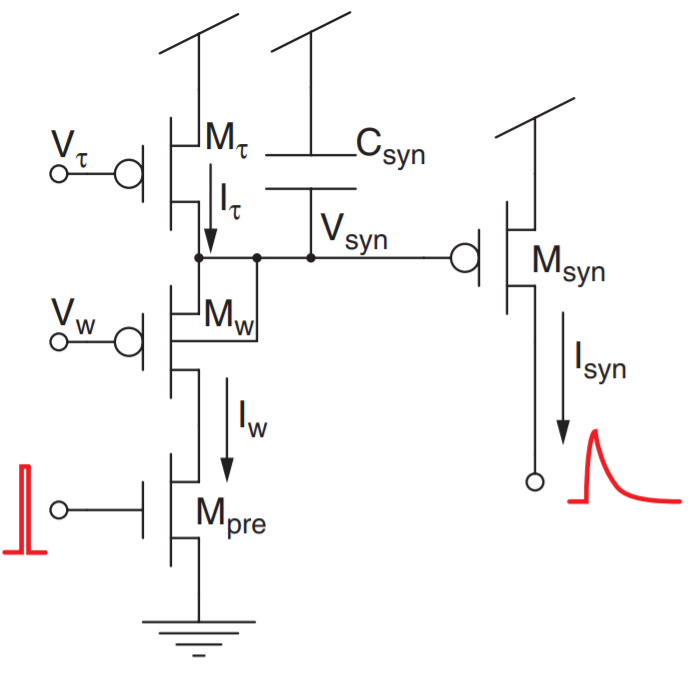
\includegraphics[width=.6\linewidth]{Figures/log_domain_pulse_integrator.PNG}
    \caption{Log-domain pulse circuit.}
    \label{fig:log_domain_pulse_integrator}
\end{figure}

A similar circuit with synaptic behaviour is the log-domain pulse integrator. It is shown in figure \ref{fig:log_domain_pulse_integrator}. The only difference compared to the previous circuit is that the transistor $M_w$ is replaced by a pFET and its n-well is now connected to the source voltage $V_{syn}$. Why do we do that? Remember from chapter \ref{sec:body_effect} that transistors are usually distorted by the body effect. By connecting the n-well to $V_{syn}$, we can cancel out this effect and thereby ensure that the thresholds of the $M_w$ and $M_{\tau}$ transistors remain similar. The updated equation of the weighted input current is:

\begin{equation}
    I_w = I_0 e^{\frac{\kappa}{U_T}(V_{syn}-V_w)}
\end{equation}

Let's try to find an analytical description for our output current $I_{syn}$. First, we want to know how our current changes over time.

\begin{equation}
    \frac{d}{dt} I_{syn} = -I_{syn} \frac{\kappa}{U_T} \frac{d}{dt} V_{syn}
\end{equation}

\begin{equation}
    \text{With } \tau = \frac{C_{syn}U_T}{\kappa I_{syn}}: \frac{d}{dt}I_{syn} = -I_{syn} \frac{\kappa}{U_T} \frac{d}{dt} V_{syn}
\end{equation}

\begin{equation}
    \text{With } I_c = I_{\tau} - I_w: \tau \frac{d}{dt} I_{syn} = - I_{syn} + I_{syn} \frac{I_w}{I_{\tau}}
\end{equation}

We can further rewrite our input current $I_w$ as follows:

\begin{equation}
    I_w = I_0 e^{-\frac{\kappa}{U_T}(V_w - V_{syn})} = I_0 e^{-\frac{\kappa}{U_T}(V_w - V_{dd})} e^{\frac{\kappa}{U_T}(V_{syn} - V_{dd})} = I_{w0} \frac{I_0}{I_{syn}}
\end{equation}

where $I_{w0}$ is the current $I_w$ at the beginning of the charge phase, i.e. when $V_{syn} = V_{dd}$. By using this new equation of $I_w$, we can get the following differential equation for our output current $I_{syn}$:

\begin{equation}
    \frac{d}{dt} I_{syn} + I_{syn} = \frac{I_0 I_{w0}}{I_{\tau}}
\end{equation}

While this circuit provides a good approximation of synaptic behaviour, it highly restricts our control of the output current $I_{syn}$. Both $I_0$ and $I_{\tau}$ are fixed values. Additionally, we have to ensure that $I_{w}$ remains in subthreshold (I w has to be large because the fixed factor is small). So how can we construct a more controllable silicon synapse?